\documentclass{article}
\usepackage[utf8]{inputenc}
\usepackage{geometry}
 \geometry{
 a4paper,
 total={170mm,257mm},
 left=20mm,
 top=20mm,
 }
 \usepackage{graphicx}
 \usepackage{titling}
 \usepackage{listings}
 \usepackage[hyphens]{url} 
\usepackage{listings}
\usepackage{xcolor}

\definecolor{codegreen}{rgb}{0,0.6,0}
\definecolor{codegray}{rgb}{0.5,0.5,0.5}
\definecolor{codepurple}{rgb}{0.58,0,0.82}
\definecolor{backcolour}{rgb}{0.95,0.95,0.92}

\lstdefinestyle{mystyle}{
    backgroundcolor=\color{backcolour},   
    commentstyle=\color{codegreen},
    keywordstyle=\color{magenta},
    numberstyle=\tiny\color{codegray},
    stringstyle=\color{codepurple},
    basicstyle=\ttfamily\footnotesize,
    breakatwhitespace=false,         
    breaklines=true,                 
    captionpos=b,                    
    keepspaces=true,                 
    numbers=left,                    
    numbersep=5pt,                  
    showspaces=false,                
    showstringspaces=false,
    showtabs=false,                  
    tabsize=2
}

\lstset{
    language=Python,
    frame=single,
    backgroundcolor=\color{lightgray},
    basicstyle=\ttfamily\footnotesize,
    keywordstyle=\color{blue},
    commentstyle=\color{green!60!black},
    stringstyle=\color{red},
    showstringspaces=false
}


 \usepackage{hyperref}
\usepackage{glossaries} % Ajout du package pour le glossaire

 \title{ChatBot Langchain pour l'UQAC}
\author{Mathis Aulagnier}
\date{\today}
 
\usepackage{hyperref}
\usepackage{fancyhdr}
\fancypagestyle{plain}{%  the preset of fancyhdr 
    \fancyhf{} % clear all header and footer fields
    \fancyfoot[L]{\thedate}
    \fancyfoot[R]{\includegraphics[width=2cm]{UQAC_Logo.png}} % Logo et numéro de page en bas à droite
    \fancyhead[L]{ChatBot Langchain pour l’UQAC}
    \fancyhead[R]{\theauthor}
}

% Appliquer le même style à toutes les pages
\pagestyle{fancy}
    \fancyhead[L]{ChatBot Langchain pour l’UQAC}
    \fancyhead[R]{\theauthor}
\fancyfoot[L]{\thedate}
\fancyfoot[R]{\includegraphics[width=2cm]{UQAC_Logo.png}} % Logo et numéro de page en bas à droite


\makeatletter
\def\@maketitle{%
  \newpage
  \null
  \vskip 1em%
  \begin{center}%
  \let \footnote \thanks
    {\LARGE \@title \par}%
    \vskip 1em%
    %{\large \@date}%
  \end{center}%
  \par
  \vskip 1em}
\makeatother

\usepackage{lipsum}  
\usepackage{cmbright}

\begin{document}

\maketitle
\noindent\begin{tabular}{@{}ll}
    Réalisé par :\\
        & Mathis Aulagnier AULM12040200 \\
        & Ryan COLLOBERT COLR28120200 \\
        & Samuel Madrigal MADS23060200 \\
    Cours :  &  8INF974 – ATELIER PRATIQUE EN INTELLIGENCE ARTIFICIELLE II \\
\end{tabular}

\section{Introduction}

L'Université du Québec à Chicoutimi (UQAC) regroupe plus de 6500 étudiants répartis dans plus de 200 programmes d'études. Pour assurer sa gestion administrative, l'université dispose d'un manuel de gestion qui regroupe l'ensemble des règlements, politiques et procédures. Face au volume croissant de ce manuel, les employés rencontrent des difficultés pour retrouver rapidement l'information nécessaire.
Dans le cadre du cours 8INF974 - Atelier pratique en intelligence artificielle II, notre équipe de trois étudiants a été mandatée pour développer une preuve de concept d'un chatbot. Ce projet s'inscrit dans une démarche d'innovation, exploitant les récentes avancées en traitement du langage naturel (NLP) et en apprentissage automatique (ML).
\subsection{Objectifs} Notre projet vise à créer un assistant conversationnel capable de répondre efficacement aux questions des employés concernant le manuel de gestion. Pour atteindre cet objectif, nous explorons la mise en œuvre de chatbots avec LangChain, intégrons l'intelligence artificielle dans une application web, et approfondissons nos connaissances dans le développement d'IA.
Notre solution s'appuie sur la technique RAG (Retrieval Augmented Generation), qui combine deux étapes clés : 
\begin{itemize} 
    \item Le Retrieval (Récupération) : recherche des informations pertinentes dans une base de données en fonction de la question posée 
    \item L'Augmented Generation (Génération Augmentée) : utilisation des informations récupérées pour enrichir le contexte et générer une réponse précise via un modèle de langage 
\end{itemize}
En combinant ces deux étapes, le RAG peut produire des réponses plus précises et contextuellement appropriées.

Pour des raisons de confidentialité et de coûts, notre solution utilise un modèle de langage hébergé localement plutôt qu'un service cloud.


\clearpage

\section{Scraping des Pages Web}

Notre approche de scraping a évolué en trois phases distinctes pour optimiser la qualité des données extraites :

\begin{enumerate}
    \item \textbf{Scraping Initial} \\
    Première approche avec un script Python basique effectuant du drill-down sur le site. Cette méthode a révélé des limitations importantes dues à la structure répétitive des pages (table des matières et sommaire redondants).

    \item \textbf{Optimisation du Script} \\
    Amélioration du script pour :
    \begin{itemize}
        \item Supporter l'extraction des fichiers PDF
        \item Cibler spécifiquement les balises "Article"
        \item Filtrer les éléments HTML indésirables
    \end{itemize}
    
    \item \textbf{Solution Finale avec Crawl4AI} \\

La découverte du dépôt \texttt{Crawl4AI} sur GitHub \href{https://github.com/unclecode/crawl4ai}{https://github.com/unclecode/crawl4ai} a été notre choix final pour le scrapping. Cette bibliothèque, spécialement conçue pour l'extraction de données destinées aux modèles de langage, offre plusieurs avantages cruciaux :

\begin{itemize}
    \item \textbf{AsyncWebCrawler} : Cette bibliothèque facilite le traitement parallèle des requêtes, ce qui diminue considérablement le temps nécessaire pour extraire les données. Sa capacité à gérer les opérations de manière asynchrone est particulièrement utile pour traiter le grand nombre de pages de notre manuel de gestion. Cependant, nous avons dû changer notre adresse IP à plusieurs reprises, car le site de l'UQAC nous a bannis en raison de l'envoi soudain d'un trop grand nombre de requêtes.
    
    \item \textbf{DefaultMarkdownGenerator} : Ce composant assure une conversion fidèle du contenu HTML/PDF en Markdown, préservant la structure des documents tout en les rendant plus accessibles pour notre chaîne de traitement RAG.
    
    \item \textbf{Le nettoyage du contenu} est optimisé grâce aux filtres préconfigurés de Crawl4AI. Notre script \texttt{getArticle.py} utilise notamment le \texttt{PruningContentFilter} avec un seuil de 0.4, permettant de:
    \begin{itemize}
        \item Isoler le contenu pertinent dans les balises "article"
        \item Supprimer les éléments de navigation redondants
        \item Éliminer les publicités et contenus non pertinents
    \end{itemize}
\end{itemize}

Ensuite, notre script \textit{getURL.py} utilise la sitemap.xml du site pour cartographier en profondeur le site. Le sitemap nous a notamment permis d'identifier plus de \textbf{293} pages pertinentes à traiter.


\end{enumerate}

\clearpage

\section{Conception de notre RAG}

\subsection{Contexte et Objectifs}
La mise en place d'un système RAG (Retrieval-Augmented Generation) nécessite une recherche approfondie sur les méthodes de construction et les optimisations possibles. Notre démarche a débuté par l'identification des formats de données les plus adaptés aux modèles de langage. Le format Markdown s'est imposé naturellement, offrant une structure claire tout en restant simple à manipuler. Cette décision a guidé notre choix d'utiliser \texttt{crawl4AI} pour l'extraction des données, nous permettant ainsi d'obtenir directement un format optimal pour la suite du traitement.

\subsection{Comparaison des Architectures de Chatbots}

\subsubsection{Le Chatbot Traditionnel}
Le chatbot basé sur un graphe représente l'approche la plus conventionnelle. Il fonctionne avec un ensemble prédéfini de questions et réponses stockées dans une base de données relationnelle. Bien que cette méthode garantisse des réponses rapides et précises pour les cas anticipés, elle souffre d'un manque crucial de flexibilité. L'impossibilité de traiter des questions non prévues limite considérablement son utilité dans des contextes dynamiques.

Voici, le schéma présentant l'architecture du chatbot traditionnel : 

\begin{figure}[ht]
    \centering
    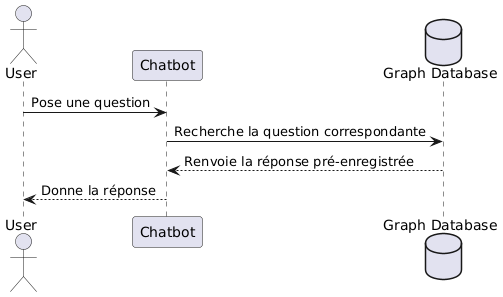
\includegraphics[width=0.5\textwidth]{chatbot_graphe.png}
    \caption{Architecture d’un chatbot basé sur un graphe}
\end{figure}

\subsubsection{L'Évolution vers les LLM}
L'introduction des modèles de langage (LLM) a marqué une évolution majeure. Ces systèmes génèrent des réponses en s'appuyant sur leur compréhension du langage naturel, acquise lors de leur entraînement. Bien que plus flexibles que leurs prédécesseurs, ils présentent une limitation importante : l'absence de connexion à des sources d'information externes actualisées. Cette caractéristique peut conduire à des réponses imprécises ou obsolètes, particulièrement dans des domaines spécialisés.

Voici, le schéma présentant l'architecture du chatbot connecté à un LLM : 
\begin{figure}[ht]
    \centering
    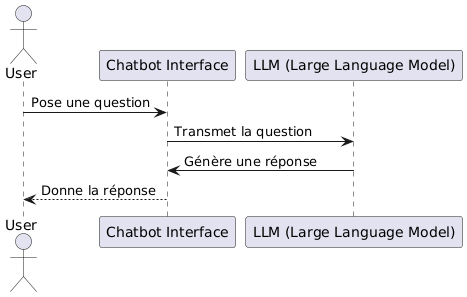
\includegraphics[width=0.5\textwidth]{LLM.png}
    \caption{Architecture d’un chatbot basé sur un LLM}
\end{figure}

\subsubsection{L'Innovation RAG}
Le système RAG représente une synthèse innovante, combinant les avantages des deux approches précédentes. En associant la puissance générative d'un LLM à une base de connaissances externe, il permet de produire des réponses à la fois contextuelles et factuellement précises. Cette architecture permet une mise à jour continue des connaissances sans nécessiter de réentraînement du modèle.

Voici, le schéma présentant l'architecture d'un RAG : 

\begin{figure}[ht]
    \centering
    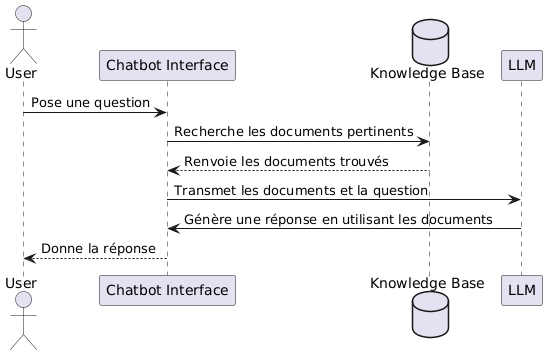
\includegraphics[width=0.5\textwidth]{RAG.png}
    \caption{Architecture d’un chatbot basé sur un RAG}
\end{figure}


\subsection{Système de Recherche Intelligent}

\subsubsection{Défis de la Recherche Documentaire}
La recherche efficace dans une base documentaire pose un défi majeur. Une approche par mots-clés simples s'avère souvent insuffisante, produisant trop de résultats sans garantie de pertinence contextuelle. Notre solution repose sur l'utilisation d'embeddings, permettant une compréhension plus profonde du contexte des requêtes.

\subsubsection{Vectorisation Sémantique}
Notre système transforme aussi bien les questions que les documents en vecteurs numériques grâce au modèle Llama3. Ces vecteurs de dimension 4096 capturent les nuances sémantiques du texte, permettant des comparaisons précises basées sur la similarité conceptuelle plutôt que sur la simple correspondance de mots.

\subsection{Innovations Techniques}

\subsubsection{Traitement et Segmentation des Données}
La gestion efficace des données extraites constitue un défi majeur dans notre architecture RAG. Les documents Markdown, bien que bien structurés, sont souvent trop volumineux pour être traités directement par les modèles de langage. Pour résoudre ce problème, nous avons implémenté un système de découpage intelligent utilisant \texttt{MarkdownTextSplitter} de Langchain. 

Cette approche permet de diviser les documents en segments (chunks) tout en préservant leur cohérence sémantique. Le système maintient un recouvrement (overlap) entre les segments consécutifs, garantissant ainsi la conservation du contexte global. Cette méthode s'est révélée particulièrement efficace pour respecter les contraintes de tokens des modèles tout en préservant l'intégrité de l'information.

\subsubsection{Enrichissement par Métadonnées}
Chaque chunk généré est enrichi avec un ensemble de métadonnées cruciales :
\begin{itemize}
    \item L'URL source du document original
    \item La position relative dans le document
    \item Les informations contextuelles essentielles
\end{itemize}
Cette structuration permet non seulement la traçabilité des informations mais facilite également la reconstitution du contexte complet lorsque nécessaire.

\subsubsection{Architecture de Stockage}
Le choix de Chroma DB comme base de données vectorielle représente un élément clé de notre architecture. Cette solution offre des capacités d'indexation et de recherche optimisées pour les vecteurs de haute dimension, garantissant des temps de réponse rapides même sur de grands volumes de données. Le processus complet suit une séquence logique :
\begin{enumerate}
    \item Prétraitement et segmentation des documents
    \item Vectorisation des chunks via Llama3
    \item Stockage structuré dans Chroma DB
\end{enumerate}

\subsubsection{Gestion Contextuelle}
Notre système maintient la cohérence des informations grâce à une gestion sophistiquée des métadonnées. Chaque fragment de texte conserve ses liens avec le document source et son contexte d'origine, permettant une reconstitution fidèle de l'information complète lorsque nécessaire.

\subsubsection{Optimisation des Performances}
L'architecture a été conçue pour équilibrer précision et rapidité. Le système de chunking intelligent, combiné à l'indexation vectorielle, permet de maintenir des temps de réponse optimaux tout en garantissant la pertinence des résultats. La taille des chunks a été choisi afin d'avoir assez d'information et assezcours pour eviter des erreur de token overflow .







\section{Implémentation du Chatbot}
\subsection{Architecture du RAG}
\begin{figure}[ht]
    \centering
    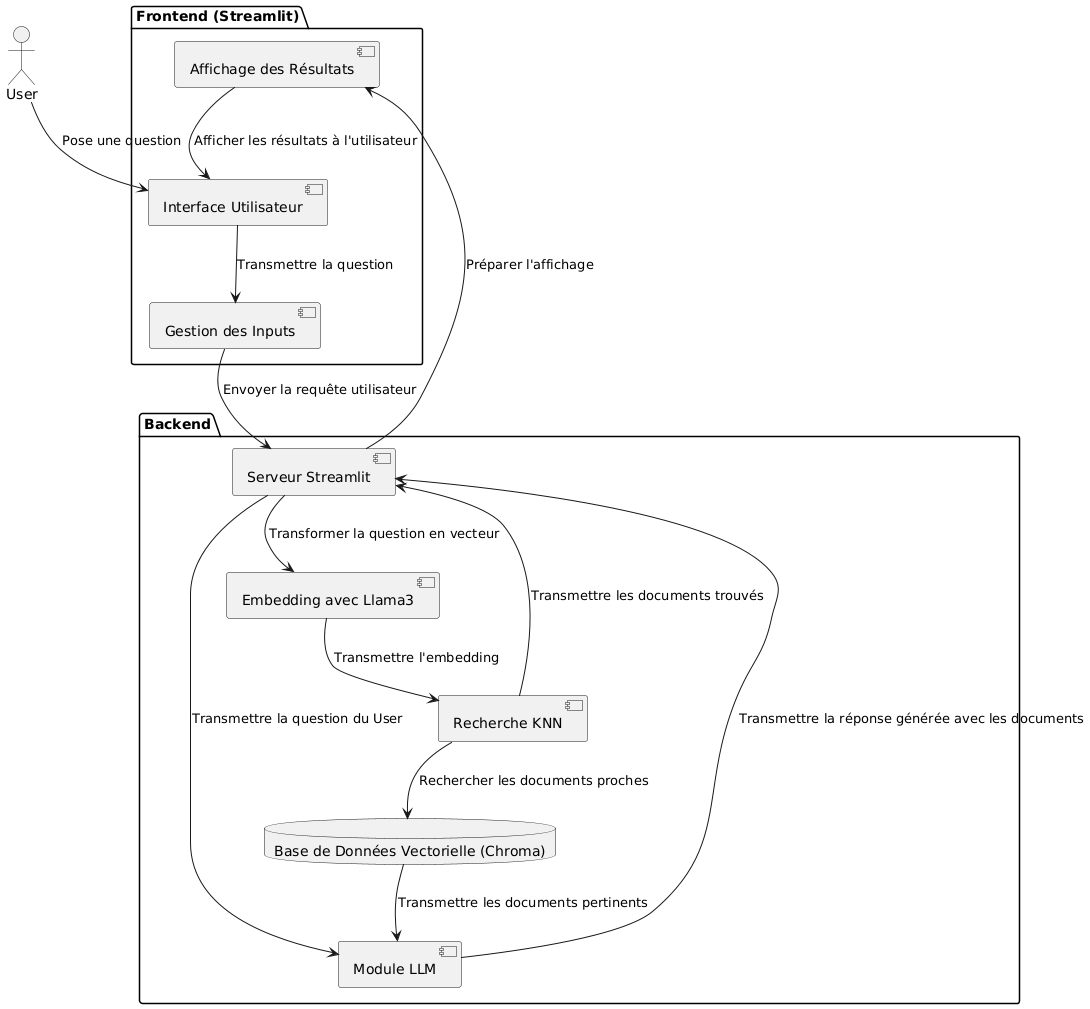
\includegraphics[width=\textwidth]{NotreRAG.png}
    \caption{Architecture d’un chatbot basé sur un RAG}
\end{figure}

\subsection{Choix du Modèle Local}


\subsection{Interface Utilisateur}


\section{Résultats}
\subsection{Performance du Système}
\subsection{Exemples de Conversations}
\subsection{Captures d'Écran}

\section{Défis et Apprentissages}
\subsection{Problèmes Rencontrés}
\subsection{Solutions Apportées}
\subsection{Améliorations Possibles}

\section{Conclusion}
\subsection{Bilan du Projet}
\subsection{Perspectives}

\end{document}